\documentclass[10pt]{article}
\pdfinfoomitdate=1
\pdftrailerid{}
\usepackage[margin=0.68in]{geometry}
\usepackage{graphicx,booktabs,array,microtype,hyperref,xcolor,amsmath,amssymb,enumitem,caption}
\usepackage[T1]{fontenc}
\usepackage{lmodern}
\definecolor{accent}{HTML}{4F6F00}
\definecolor{soft}{HTML}{F4F7EE}
\hypersetup{colorlinks=true,linkcolor=accent,citecolor=accent,urlcolor=accent}
\setlist{nosep,leftmargin=*}
\setlength{\parindent}{0pt}
\setlength{\parskip}{4pt}
\title{\vspace{-1.1em}\textbf{BeliefWeave: Governing When Memory May Change Behavior}}
\author{Aura Yavary}
\date{}
\begin{document}
\maketitle

\begin{abstract}
Long-term personalization is usually evaluated as a memory retrieval problem: can an assistant recover the right fact from a long interaction history? We study a different failure mode. A memory can be retrieved correctly and still be unsafe or inappropriate to use because it is stale, weakly inferred, context-specific, contradicted, or superseded. We call the missing decision \emph{behavioral authority}. BeliefWeave represents personal memory as a temporal belief state and inserts an explicit authority policy between retrieval and generation. For each candidate memory, the policy chooses \texttt{USE}, \texttt{ASK}, or \texttt{ABSTAIN}. We formalize this choice as cost-sensitive decision-making under uncertainty and evaluate it with BeliefShiftBench-v2, a frozen 320-case held-out test split spanning eight controlled failure families. BeliefWeave reaches 96.9\% exact three-way action accuracy (95\% bootstrap CI: 95.0--98.8) versus 62.5\% for a temporal-plus-context baseline and 37.5\% for retrieval-only; false personalization falls from 62.5\% to 1.6\%. A paired exact McNemar test against temporal-plus-context gives $p<10^{-32}$. Controlled response interventions yield 98.4\% personalization-intervention fidelity. Fault injection shows that incorrect state lifecycle and source attribution are the largest upstream failure amplifiers. A 10,000-turn local memory-core stress test maintains zero duplicate active single-valued slots with sub-millisecond p95 memory updates in the tested environment. These results are controlled synthetic evidence, not a claim of real-user utility or broad state of the art. A separate post-hoc unseen-composition challenge deliberately leaves the v2 template families and drops the original gate to 75.0\% exact accuracy, exposing three specification gaps (future-effective beliefs, unknown current context for scoped memories, and synthetic evidence). A challenge-informed patch closes those cases, but we do not count its score as independent generalization evidence. To make the remaining boundary executable rather than rhetorical, we include adapters/contracts for LongMemEval, PersonaMem, and OP-Bench comparison planning, plus a blind human-evaluation protocol, but report no external or human score until those studies are actually run.
\end{abstract}

\section{Introduction}
A memory system can retrieve the right sentence and still produce the wrong personalized behavior. Consider a user who once liked a food but later changed preference; a statement attributed to a friend; a preference that applies only at work; a tentative inference from one interaction; or two memories that conflict. Each item may be lexically or semantically relevant to a new request. Relevance alone does not answer whether the assistant should act on it.

This distinction matters because recent memory research increasingly succeeds at retrieval, temporal organization, and user-state inference. LongMemEval measures extraction, cross-session reasoning, temporal reasoning, knowledge updates, and abstention \cite{wu2025longmemeval}; PersonaMem evaluates evolving user profiles and personalized responses \cite{jiang2025personamem}; Zep/Graphiti maintains temporally valid knowledge graphs \cite{rasmussen2025zep}; Memora explicitly measures forgetting and reuse of invalid memories \cite{uddin2026memora}; QUMem performs query-conditioned user-state inference over evolving preferences \cite{wang2026qumem}; PAHF studies continual personalization under preference drift with clarification and feedback \cite{liang2026pahf}; and OP-Bench formalizes over-personalization and proposes Self-ReCheck memory filtering \cite{hu2026opbench}. These systems make a simple ``temporal memory'' or ``knowing when not to personalize'' claim insufficient.

We instead ask a narrower question: \textbf{when does a retrieved memory have enough authority to change downstream behavior?} BeliefWeave separates four concepts that are often collapsed: evidence, belief, retrieval relevance, and behavioral authority. The system can retrieve a memory yet abstain from using it, or ask the user before personalizing.

Our contributions are:
\begin{enumerate}
\item \textbf{Behavioral authority as a decision problem.} We formalize memory use as a three-way cost-sensitive decision under uncertainty over the user's current state.
\item \textbf{BeliefWeave.} A temporal memory substrate with validity, provenance, confidence, context, verification, conflict state, supersession, and explicit \texttt{USE}/\texttt{ASK}/\texttt{ABSTAIN} gating.
\item \textbf{BeliefShiftBench-v2.} A deterministic 640-case controlled benchmark with a frozen 320-case held-out test split and exact three-way policy labels across eight failure families.
\item \textbf{Counterfactual evaluation.} Counterfactual Personalization Regret (CPR) and intervention fidelity measure not merely whether a memory is recalled, but whether it changes behavior exactly when it should.
\item \textbf{Mechanism analysis.} Stronger metadata baselines, bootstrap confidence intervals, paired significance testing, threshold and cost sensitivity, calibration, component ablations, controlled fault injection, metamorphic invariants, benchmark mutation testing, and 10k-turn memory-core scaling.
\end{enumerate}

\section{Problem Formulation}
Let $z_t$ denote the latent current user state at time $t$ and $o_{1:t}$ the observed interaction history. A personalized system maintains a belief state
\[
 b_t(z)=P(z_t=z\mid o_{1:t}).
\]
A retrieval system returns candidate memories $m_i$ conditioned on current request $x_t$. We introduce a separate variable $y_i\in\{0,1\}$ indicating whether memory $m_i$ should be allowed to influence the current response. BeliefWeave estimates
\[
 p_i=P(y_i=1\mid m_i,x_t,b_t),
\]
then chooses an action $a_i\in\{\mathrm{USE},\mathrm{ASK},\mathrm{ABSTAIN}\}$.

\subsection{Cost-sensitive authority}
For costs $C_{FP}$ (false personalization), $C_{MISS}$ (missed useful personalization), and $C_{ASK}$ (clarification), the expected losses are
\begin{align*}
L(\mathrm{USE}) &= (1-p_i)C_{FP},\\
L(\mathrm{ABSTAIN}) &= p_i C_{MISS},\\
L(\mathrm{ASK}) &= C_{ASK}.
\end{align*}
The Bayes action is
\[
 a_i^*=\arg\min_a L(a).
\]
The implementation also includes a threshold policy used in the main BeliefWeave system. We report both because the cost-sensitive form makes the decision semantics explicit while the threshold form exposes the engineering policy currently used by the prototype.

\subsection{Memory representation}
A memory record stores value/type, source provenance, confidence, temporal validity, context scope, lifecycle state, source-event references, user verification, and conflict/supersession relations. Event $\neq$ observation $\neq$ belief $\neq$ active user state. This separation lets the system retain provenance while retiring obsolete beliefs.

\begin{center}
\fcolorbox{accent}{soft}{\parbox{0.94\linewidth}{\centering
interaction $\rightarrow$ immutable event $\rightarrow$ candidate observation $\rightarrow$ write/abstain $\rightarrow$ typed temporal memory $\rightarrow$ state update $\rightarrow$ retrieval $\rightarrow$ \textbf{authority decision} $\rightarrow$ generation}}
\end{center}

\section{BeliefWeave}
\subsection{Temporal state maintenance}
Memories have explicit validity and lifecycle status. Expired, superseded, deleted, or context-incompatible records can remain auditable without appearing in the active state. Multi-valued preferences and goals are additive by default; destructive replacement requires structurally compatible evidence. Explicit corrections can supersede prior beliefs.

\subsection{Provenance and conflict}
The writer distinguishes explicit, observed, inferred, and other source types. Role-play, hypothetical statements, third-party attribution, and explicit ``do not remember'' instructions are guarded before durable persistence. A learned conflict classifier is bounded by structural rules so unrelated memory types cannot silently overwrite each other.

\subsection{Authority estimation}
The transparent authority estimator begins from memory confidence, then adjusts for provenance and user verification. Hard lifecycle invalidity maps authority near zero; context mismatch sharply suppresses it; unresolved conflict maps to maximal uncertainty rather than silent use. This is intentionally inspectable. We do not claim that these hand-designed features are a final calibrated probability model.

\section{Evaluation Design}
\subsection{BeliefShiftBench-v2}
The benchmark contains 640 controlled cases across eight families: valid explicit evidence, valid observed evidence, stale memory, context mismatch, weak inference, unresolved conflict, inactive/superseded memory, and medium-authority evidence. The first 320 cases form a development split and the remaining 320 form a frozen held-out test manifest. The two splits share failure families but use disjoint case IDs and parameter values. Thus the test split prevents direct per-item tuning, but it is still author-constructed synthetic data rather than independent annotation.

Gold labels are three-way actions, not merely ``use vs. do not use.'' Valid evidence maps to \texttt{USE}; unresolved conflicts and medium-authority evidence map to \texttt{ASK}; stale, inactive, context-mismatched, and weakly inferred evidence map to \texttt{ABSTAIN}.

\subsection{Baselines}
We compare against: (1) retrieval-only use of every active memory, (2) confidence thresholding, (3) provenance-only filtering, (4) temporal-plus-context filtering, (5) an additive metadata score without hard vetoes, (6) the explicit cost-sensitive Bayes policy, and (7) an oracle upper bound. These baselines are stronger than the original retrieval-only comparison but remain local metadata policies rather than full external memory systems.

\subsection{Metrics and statistics}
We report exact three-way action accuracy, binary use accuracy, false-personalization rate, use precision/recall, ask/abstain rates, and CPR. Main metrics receive 1,000-sample bootstrap 95\% confidence intervals. We use exact paired McNemar tests on per-case action correctness when comparing BeliefWeave with deterministic baselines.

For a memory intervention, let $Y(M)$ be the response behavior with memory set $M$ and $Y(M\setminus\{m\})$ the counterfactual after removing $m$. Personalization intervention fidelity is the fraction of cases in which personalized content changes if and only if $m$ is gold-authoritative. A second behavior-level fidelity treats a warranted clarification as an intentional behavior change.

\subsection{Additional controlled probes}
We run: (i) threshold and cost sensitivity, (ii) calibration and risk-coverage analysis, (iii) leave-one-signal-out authority ablations, (iv) controlled upstream fault injection, (v) memory-core scaling at horizons 10, 100, 1,000, and 10,000 turns, (vi) a 30-seed stochastic metadata stress test, and (vii) a structurally novel composition challenge that is explicitly excluded from parameter tuning. The repository also retains the earlier 100k-interaction generated corpus, retrieval ranking suite, OOD observation-router suite, and regression/invariant tests.

\section{Main Results}
\begin{table}[t]
\centering\small
\caption{Held-out BeliefShiftBench-v2 test results ($n=320$). CI is bootstrap 95\% CI for exact action accuracy. CPR is lower-is-better.}
\begin{tabular}{lrrrr}
\toprule
Policy & Exact acc. & 95\% CI & False pers. & CPR \\
\midrule
Retrieval-only & 37.5 & [32.5, 42.8] & 62.5 & 1.250 \\
Confidence-only & 50.0 & [44.1, 55.6] & 37.5 & 0.750 \\
Provenance-only & 50.0 & [44.1, 55.6] & 50.0 & 1.000 \\
Temporal + context & 62.5 & [56.9, 68.1] & 37.5 & 0.750 \\
Metadata score, no hard veto & 59.4 & [53.8, 65.0] & 39.1 & 0.813 \\
Cost-sensitive authority & 83.1 & [79.1, 87.2] & \textbf{0.0} & 0.105 \\
\textbf{BeliefWeave} & \textbf{96.9} & \textbf{[95.0, 98.8]} & 1.6 & \textbf{0.094} \\
Oracle & 100.0 & [100, 100] & 0.0 & 0.063 \\
\bottomrule
\end{tabular}
\end{table}

BeliefWeave improves exact three-way policy accuracy by 34.4 points over temporal-plus-context filtering. In paired testing, BeliefWeave is correct on 110 cases where temporal-plus-context is wrong and loses on zero cases, yielding exact two-sided McNemar $p=1.54\times10^{-33}$. Against the metadata-score baseline the corresponding discordant counts are 120 versus zero ($p=1.50\times10^{-36}$). These extremely small p-values reflect the deterministic controlled construction and should not be interpreted as evidence of external generalization.

\begin{figure}[t]
\centering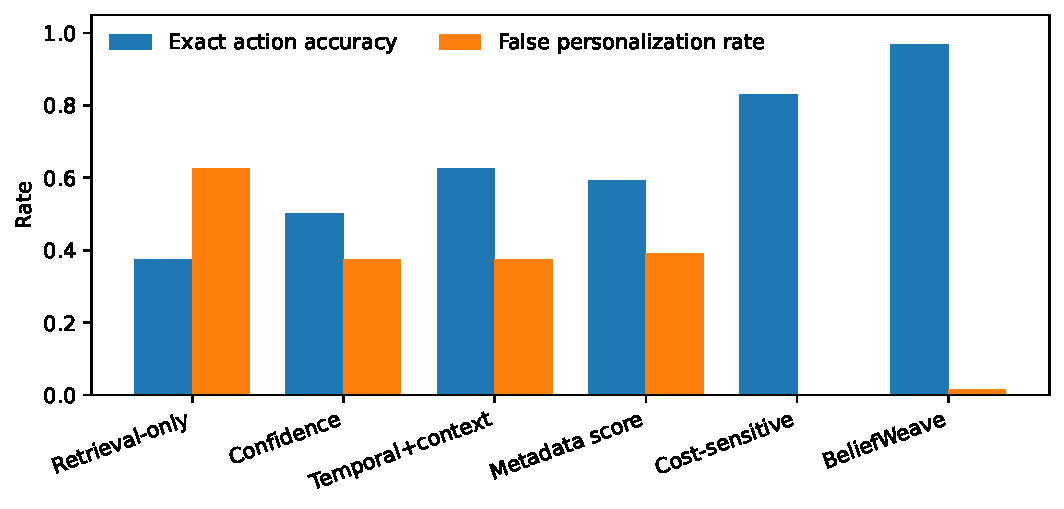
\includegraphics[width=.82\linewidth]{figures/authority_baselines.pdf}
\caption{Three-way action accuracy and false-personalization rate on the frozen synthetic test split.}
\label{fig:authority}
\end{figure}

\subsection{Calibration and selective personalization}
The raw authority score obtains Brier score 0.118, NLL 0.333, ECE 0.224, and adaptive ECE 0.210 on the held-out synthetic split. This is a useful negative result: the score orders evidence reasonably enough for gating, but should not yet be interpreted as a well-calibrated probability. Figure~\ref{fig:riskcoverage} reports the false-use risk as acceptance coverage changes. A production system should calibrate $p_i$ on independent behavioral-authority labels rather than reuse the current heuristic score.

\begin{figure}[h]
\centering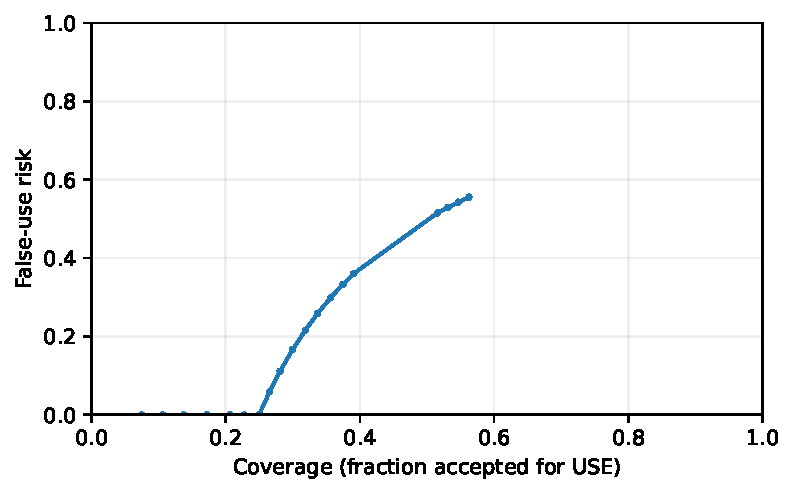
\includegraphics[width=.57\linewidth]{figures/risk_coverage.pdf}
\caption{Risk-coverage curve for accepting memories as behaviorally authoritative.}
\label{fig:riskcoverage}
\end{figure}

\subsection{Component ablations}
The cost-sensitive policy provides a clean mechanism probe because each metadata signal can be removed without changing the rest of the decision rule. Removing time or context raises CPR from 0.105 to 0.355; removing conflict handling raises it to 0.323. Removing lifecycle status causes all inactive-memory cases to fail. Provenance has a smaller aggregate effect in this controlled mix, while user verification is redundant for the current cost rule. This last result is informative rather than desirable: the benchmark does not yet contain enough near-boundary verified cases to identify a verification contribution.

\begin{figure}[h]
\centering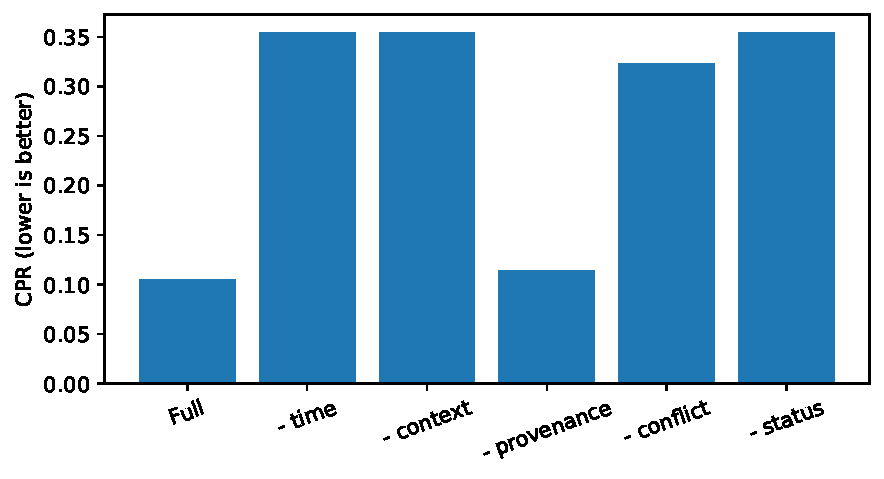
\includegraphics[width=.66\linewidth]{figures/authority_ablation_v2.pdf}
\caption{Counterfactual Personalization Regret under signal ablations.}
\label{fig:ablation}
\end{figure}

\subsection{Sensitivity, stochastic stability, and unseen compositions}
The threshold sweep contains 168 $(\tau_{\mathrm{use}},\tau_{\mathrm{ask}})$ settings. Exact action accuracy ranges from 76.3\% to 100\%; only 8 settings (4.8\%) lie within one percentage point of the best setting. Across 60 cost triples, exact accuracy ranges from 56.3\% to 84.4\%, and only 20\% of settings simultaneously exceed 80\% exact accuracy and stay below 5\% false personalization. This is evidence that the normative trade-off is genuinely consequential rather than a cosmetic hyperparameter.

A separate stochastic suite samples label-safe confidence/provenance/context values for 400 cases per seed across 30 seeds (12,000 decisions per policy). BeliefWeave remains at 100\% exact action accuracy in this within-specification perturbation, while the cost-sensitive authority baseline averages 89.5\% with roughly 1.0 percentage point standard deviation. This stability result should not be confused with distribution shift.

To test specification shift, we designed a post-hoc unseen-composition challenge containing future-effective beliefs, scoped memories with unknown current context, synthetic high-confidence evidence, and other combinations absent from BeliefShiftBench-v2. The original gate reaches only 75.0\% exact accuracy across 2,880 decisions; all errors concentrate in the three previously unsupported conditions. Figure~\ref{fig:unseen} makes the gap explicit. We then implemented a separate \texttt{DecisionAwareBeliefGateV2} with conservative rules for those conditions. It reaches 100\% on the same challenge, but because the patch was motivated by observing the failures, that number is treated only as a regression result and not as independent evidence.

After freezing that V2 patch, we constructed a second 480-case specification audit before writing any further patch. V2 reaches only 53.3\% exact accuracy. Seven complete families fail: inactive or expired scoped memories are incorrectly routed to clarification when context is unknown; malformed temporal metadata is allowed to personalize; missing provenance is ignored; and sensitive unverified memory is used without confirmation. We then implemented a separate V3 hardening pass that fixes these cases; its 100\% score on the same audit is again reported only as regression evidence. Importantly, both V2 and V3 pass 185/185 metamorphic monotonicity/safety checks, while BeliefShiftBench-v2 kills 6/6 intentionally corrupted authority implementations. These results separate three questions that raw accuracy conflates: within-specification consistency, benchmark fault sensitivity, and true generalization beyond the authored specification.

\begin{figure}[h]
\centering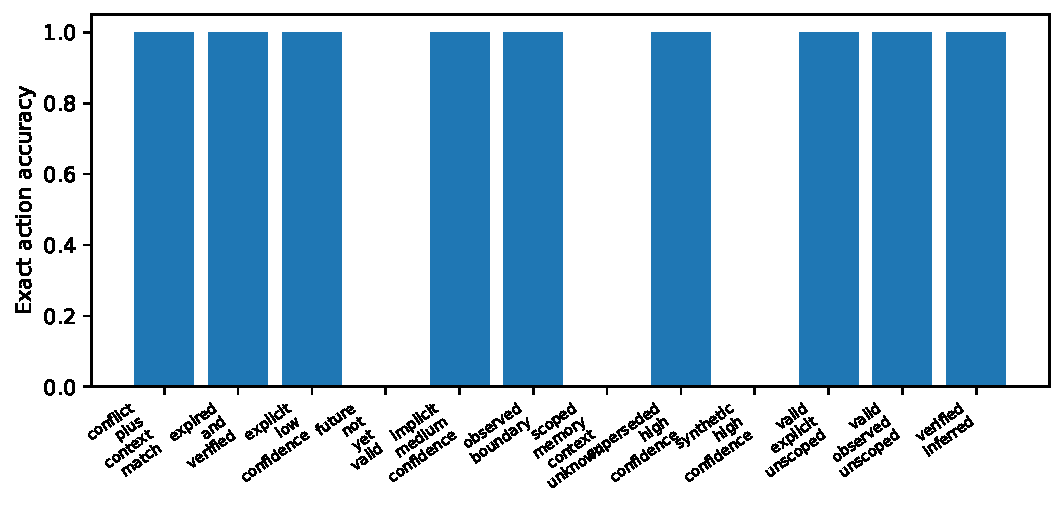
\includegraphics[width=.94\linewidth]{figures/unseen_composition.pdf}
\caption{Post-hoc unseen-composition challenge for the original gate. Zero bars identify specification gaps rather than random noise.}
\label{fig:unseen}
\end{figure}

\begin{figure}[h]
\centering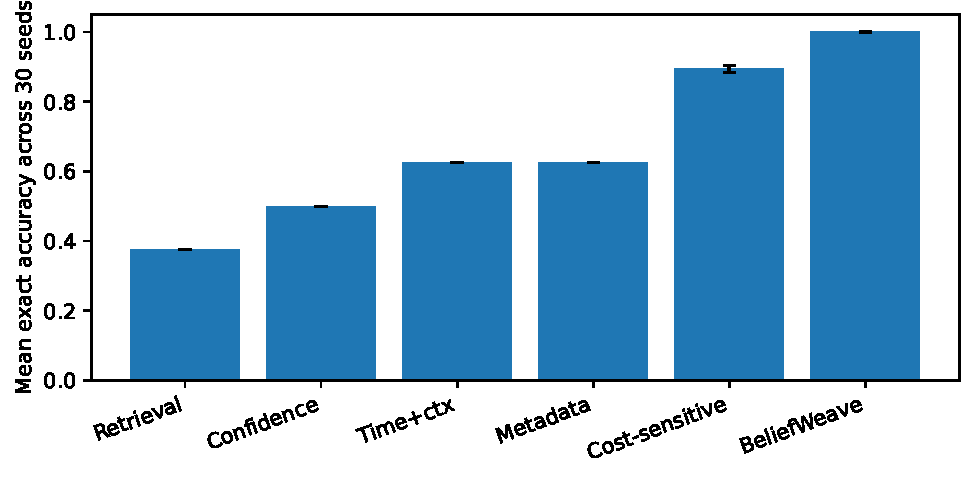
\includegraphics[width=.80\linewidth]{figures/stochastic_stability.pdf}
\caption{Thirty-seed stochastic perturbation within pre-specified label-safe ranges. Error bars are standard deviations across seeds.}
\label{fig:stability}
\end{figure}

\subsection{Counterfactual response intervention}
A deterministic response renderer isolates whether memory changes generated content at all, without confounding the experiment with an external LLM. BeliefWeave reaches 98.4\% personalization-intervention fidelity and 98.4\% behavior-intervention fidelity, with 1.6\% false personalization influence. Retrieval-only reaches 37.5\% personalization-intervention fidelity and 62.5\% behavior-intervention fidelity. This experiment establishes causal wiring of the memory gate; it is \emph{not} evidence that free-form LLM responses are better.

\subsection{Fault propagation}
Controlled corruption exposes where upstream mistakes are amplified. Clean exact policy accuracy is 96.9\%. Corrupting source type/confidence reduces it to 75.0\%; forcing inactive/stale state back to active reduces it to 71.9\%; removing context or conflict signals yields 84.4\%. Forcing every retrieved memory to \texttt{USE} yields 25.0\%, and inverting the final authority action yields 0\%. This decomposition motivates separate evaluation of extraction, state revision, retrieval, authority, and generation rather than one end-to-end number.

\subsection{Long-horizon memory-core scaling}
The local SQLite memory core was exercised at 10, 100, 1,000, and 10,000 interaction turns with a 2\% durable-memory rate. At 10,000 turns it stores 200 historical memories and 25 active single-valued slots with zero duplicate active slots. In this environment, p95 memory update latency is 0.71 ms and p95 authority-gate latency is 0.009 ms. These numbers isolate local persistence/update/gating and exclude model inference, embedding, and network latency.

\begin{figure}[h]
\centering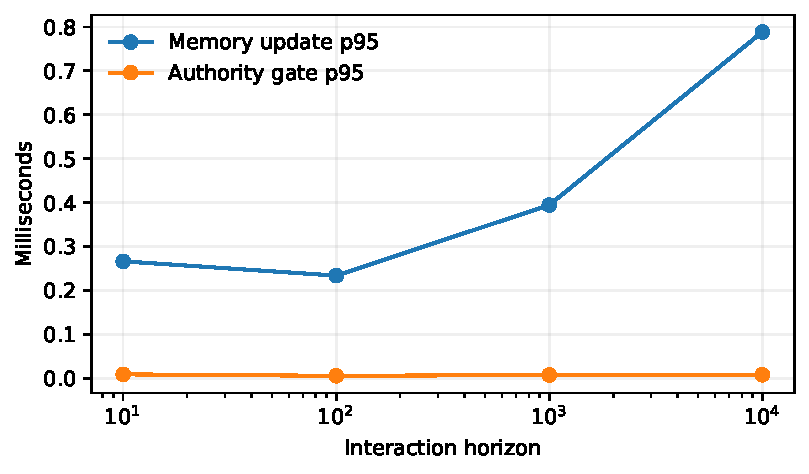
\includegraphics[width=.58\linewidth]{figures/horizon_scaling.pdf}
\caption{Local memory-core scaling. Runtime values are environment-dependent.}
\label{fig:scale}
\end{figure}

\section{Relation to Existing Memory Evaluation}
The central difference between BeliefWeave and retrieval-focused evaluation is the target variable. LongMemEval asks whether a system can retrieve and reason over long interaction histories \cite{wu2025longmemeval}; LongMemEval-V2 extends this to environment-specific experience for web agents \cite{wu2026longmemevalv2}. PersonaMem asks whether models infer evolving profiles and generate personalized responses \cite{jiang2025personamem}, while PersonaMem-v3 explicitly adds over-personalization and restraint, including cases where personalization is inappropriate, outdated, unnecessary, or privacy-sensitive \cite{jiang2026personamemv3}. Zep/Graphiti emphasizes temporally valid graph memory \cite{rasmussen2025zep}. Memora introduces forgetting-aware evaluation and reports frequent reuse of invalid memories \cite{uddin2026memora}. PAHF includes pre-action clarification and post-action feedback for continual preference adaptation \cite{liang2026pahf}. QUMem plans query-conditioned retrieval and infers a current user state \cite{wang2026qumem}. DCPM tracks belief trajectories and higher-level cognitive memory \cite{fei2026dcpm}. Recent conversational evaluation also finds that retrieval quality does not fully translate into response quality \cite{chang2026locomoconv}.

OP-Bench formalizes over-personalization as irrelevance, repetition, and sycophancy, and proposes Self-ReCheck, a model-agnostic memory filter that reconsiders retrieved memories before response generation \cite{hu2026opbench}. This is the closest conceptual overlap to our motivation. BeliefWeave therefore does not claim that filtering unnecessary memories or avoiding over-personalization is new. Its narrower target is an explicit, auditable \emph{per-memory authority action} after retrieval/state inference, with a three-way \texttt{USE}/\texttt{ASK}/\texttt{ABSTAIN} decision, explicit decision costs, and counterfactual intervention tests of whether a memory changed behavior when it should.\par

PersonaMem-v3 means that \emph{restraint itself is not a novelty claim}. BeliefWeave's narrower contribution is to expose restraint as an explicit memory-level decision surface \emph{after retrieval and state inference}: each candidate memory receives an auditable \texttt{USE}/\texttt{ASK}/\texttt{ABSTAIN} decision under explicit costs, and its causal influence can be tested by intervention. This is also why external evaluation is necessary. The repository includes LongMemEval/PersonaMem-family adapters and public schema contracts, but no external score is reported because third-party data/model execution was unavailable in the build environment. Reporting a fabricated proxy would weaken rather than strengthen the paper.

\section{Failure Analysis}
Several implementation failures changed the design. Simulation-time expiry initially leaked wall-clock assumptions. Third-party statements could be attributed to the user. A learned conflict classifier attempted to supersede an unrelated preference with a goal. Multi-valued preferences risked destructive collapse. Role-play could leak into memory. A calibration binning bug distorted confidence analysis. An authority-ablation fixture labeled a case stale while placing its expiry after the synthetic evaluation time. Each failure was converted into a regression test, structural guard, or benchmark correction.

The most important remaining failure is not hidden: the lightweight observation router reaches only 65.8\% accuracy on held-out paraphrase families. That weakness sits upstream of otherwise strong governance results. A better authority policy cannot recover a belief that was extracted incorrectly. The fault-injection experiment quantifies this dependence and argues for reporting stage-wise error propagation.

\section{Human and External Evaluation Protocol}
A blind human protocol is included but not populated with invented judgments. Each rater compares anonymized responses generated from the same user history/current request and answers: which response matches the current preference, which uses outdated information, which is more intrusive, whether clarification was warranted, and overall preference. Primary outcomes are pairwise preference, stale-memory harm, unsupported-personalization rate, clarification appropriateness, and intrusiveness, with confidence intervals and agreement statistics for multi-rater subsets.

For external evaluation, the LongMemEval adapter computes evidence-session recall using the benchmark's official \texttt{answer\_session\_ids}; official answer-quality evaluation still requires a reader model and official evaluator. The PersonaMem-v1 adapter creates provider-neutral model requests from the released benchmark format; the external registry also records PersonaMem-v3 as the highest-priority restraint/over-personalization target for a future full model run. These harnesses turn missing evidence into an executable next step without pretending that the run has already happened.

\section{Limitations}
The main results are generated from author-constructed synthetic cases. A frozen held-out split reduces direct per-item tuning leakage but shares scenario families with development data and therefore does not constitute template-held-out generalization. The first unseen-composition challenge drops the original gate to 75.0\%; a second pre-patch specification audit drops V2 to 53.3\%, directly demonstrating that author-designed held-out accuracy does not imply specification completeness. Baselines are stronger than retrieval-only but are not full reimplementations of Mem0, Zep, QUMem, or other external systems. The counterfactual renderer is deterministic rather than a frontier LLM. The authority score is not well calibrated. Cost weights are normative choices; sensitivity analysis is included, but the right trade-off should ultimately be estimated from user preferences and product risk. Multilingual evidence is limited. There is no completed human-subject longitudinal study, no production privacy/legal review, and no external benchmark score in this artifact. The checked-in runtime defaults to the challenge-hardened V3 policy while retaining V1/V2 for frozen reproduction; a finite 9,600-state policy audit finds zero declared-property violations for V3, but this is engineering assurance rather than independent empirical evidence.

The paper therefore supports a mechanism claim: separating retrieval from authority materially improves controlled decisions under designed temporal/provenance/conflict failures. It does not yet support a claim that BeliefWeave is the best real-world personalized memory system.

\section{Conclusion}
Personalization has a decision problem hidden inside its memory problem. A fact can be remembered correctly and still lack permission to influence the present. BeliefWeave makes that decision explicit, auditable, and measurable. The current evidence shows large controlled gains over progressively stronger metadata baselines, identifies which state signals matter, and exposes calibration and extraction weaknesses. The next decisive evidence is external: head-to-head OP-Bench/Self-ReCheck, LongMemEval-V2/PersonaMem-v3 model runs, and blind human judgments of downstream personalized responses.

\appendix
\section{Reproducibility and Artifact Boundary}
The repository contains the frozen test manifest, benchmark generators, all result JSON, figure-generation scripts, package/API tests, data-contract checks, checksums, Croissant-style benchmark metadata, external benchmark adapters, and a human-evaluation kit. No project date is embedded in the public manuscript. Bibliographic years remain because they identify cited work.


\section{Submission Readiness and Responsible Dataset Metadata}
The repository includes a pre-submission NeurIPS checklist, human-evaluation power planning, an explicit list of external evidence still required before broad claims, and Croissant metadata with core plus minimal Responsible-AI fields. The local Croissant checker verifies field presence and structure. A reviewer-accessible hosted dataset URL and the official network Croissant validator cannot be completed inside the offline build and are therefore recorded as submission-time external actions rather than falsely marked complete.

\section{Original Retrieval and OOD Diagnostics}
The earlier retrieval suite contains 120 controlled queries. Hybrid local retrieval improves Hit@1 from 55.0\% to 73.3\%, Hit@3 from 86.7\% to 95.0\%, and MRR from 0.683 to 0.835, with zero stale-memory leaks in that suite. The observation router reaches 65.79\% on 114 held-out paraphrase examples; at confidence threshold 0.70 it reaches 83.78\% selective accuracy at 32.46\% coverage. These results remain supporting diagnostics rather than the headline authority result.

\begin{thebibliography}{20}
\bibitem{park2023generative} J. S. Park et al. \emph{Generative Agents: Interactive Simulacra of Human Behavior}. 2023.
\bibitem{maharana2024locomo} A. Maharana et al. \emph{Evaluating Very Long-Term Conversational Memory of LLM Agents}. ACL, 2024.
\bibitem{wu2025longmemeval} D. Wu, H. Wang, W. Yu, Y. Zhang, K.-W. Chang, and D. Yu. \emph{LongMemEval: Benchmarking Chat Assistants on Long-Term Interactive Memory}. ICLR, 2025.
\bibitem{jiang2025personamem} B. Jiang et al. \emph{Know Me, Respond to Me: Benchmarking LLMs for Dynamic User Profiling and Personalized Responses at Scale}. COLM, 2025.
\bibitem{rasmussen2025zep} P. Rasmussen, P. Paliychuk, T. Beauvais, J. Ryan, and D. Chalef. \emph{Zep: A Temporal Knowledge Graph Architecture for Agent Memory}. arXiv:2501.13956, 2025.
\bibitem{liang2026pahf} K. Liang et al. \emph{Learning Personalized Agents from Human Feedback}. arXiv:2602.16173, 2026.
\bibitem{uddin2026memora} M. N. Uddin, K. Shubham, E. Blanco, C. Baral, and G. Wang. \emph{From Recall to Forgetting: Benchmarking Long-Term Memory for Personalized Agents}. arXiv:2604.20006, 2026.
\bibitem{fei2026dcpm} T. Fei, M. Song, M. Zheng, and X. Yu. \emph{Memory Beyond Recall: A Dual-Process Cognitive Memory System for Self-Evolving LLM Agents}. arXiv:2606.09483, 2026.
\bibitem{wang2026qumem} H. Wang et al. \emph{QUMem: Personalized Memory for Query-Conditioned User-State Inference in LLM Agents}. arXiv:2608.16168, 2026.
\bibitem{wu2026longmemevalv2} D. Wu, Z. Ji, A. Kawatkar, B. Kwan, J.-C. Gu, N. Peng, and K.-W. Chang. \emph{LongMemEval-V2: Evaluating Long-Term Agent Memory Toward Experienced Colleagues}. arXiv:2605.12493, 2026.
\bibitem{jiang2026personamemv3} B. Jiang et al. \emph{PersonaMem-v3: Toward Omni-Platform Personal Intelligence for Holistic User Understanding, Recommendation, and Agentic Tasks}. arXiv:2608.21381, 2026.
\bibitem{chang2026locomoconv} W.-Y. Chang and Y.-N. Chen. \emph{When Users Don't Ask: Benchmarking Context-Driven Memory Retrieval in Conversational Agents}. arXiv:2609.03467, 2026.
\bibitem{hu2026opbench} Yulin Hu, Zimo Long, Jiahe Guo, Xingyu Sui, Xing Fu, Weixiang Zhao, Yanyan Zhao, and Bing Qin. OP-Bench: Benchmarking Over-Personalization for Memory-Augmented Personalized Conversational Agents. arXiv:2601.13722, 2026.
\end{thebibliography}
\end{document}
